\section{Results}
\label{sec:results}

In this section we evaluate the \lloid{} algorithm using our \gstreamer{}-based implementation described in the previous section. We calculate the
measured \SNR\ loss due to the approximations of the \lloid\ method and our
implementation of it. Using settings that give acceptable \SNR{} loss for
our chosen parameter space, we then compute the operation counts.

\subsection{Setup}

We examine the performance of the \lloid\ algorithm on a small region of
compact binary parameter space centered on typical \textsc{ns}--\textsc{ns}
masses.  We begin by constructing a template bank that spans component masses
between 1~and~3~$M_\odot$ using a simulated Advanced \LIGO{} noise
curve~\citep{ALIGONoise}.  Then we create sub-banks by partitioning the parameter
space by chirp mass.  Figure \ref{fig:tmpltbank} illustrates this procedure.
\begin{figure}[h]
	\plotone{figures/tmpltbank.png}
	\caption{\label{fig:tmpltbank}Placement of template parameters used in this paper.  The template bank consists of 98544 templates with component masses $m_1$, $m_2$, between 1~and~3~$M_\odot$.  We design a filter bank to search for a subset of 657 of these templates with chirp masses $\mathcal M$ between 1.1955~and~1.2045~$M_\odot$.}
\end{figure}
The result is that we obtain 657 templates with chirp masses between 1.1955~and~1.2045~$M_\odot$.  With this
sub-bank we were able to construct an efficient time-slice decomposition that consisted of 11 time slices
with sample rates between 32 and 4096 Hz shown in table \ref{tab:time_slices}.
\begin{table*}
\begin{center}
\caption{\label{tab:time_slices} Filter design for these 657 templates.  From left to right, this table shows the sample rate, time interval, number of samples, and number of orthogonal templates for each time slice.  We vary \SVD{} tolerance from $\left(1-10^{-1}\right)$ to $\left(1-10^{-6}\right)$.}
\begin{tabular}{rr@{,\,}lc*{6}{r}}
\tableline\tableline
\\ [-1.5ex]
\multicolumn{4}{c}{} &\multicolumn{6}{c}{$\log_{10}$ (1$-$\SVD{} tolerance)} \\ [1ex]
\cline{5-10}
\\ [-1.5ex]
$f^s$ (Hz) & $[t^s$&$t^{s+1})$ (s) & $N^s$ & $-1$ & $-2$ & $-3$ & $-4$ & $-5$ & $-6$ \\ \tableline
4096 & [0&0.5) & 2048 & 1 & 4 & 6 & 8 & 10 & 14 \\
512 & [0.5&4.5) & 2048 & 2 & 6 & 8 & 10 & 12 & 16 \\
256 & [4.5&12.5) & 2048 & 2 & 6 & 8 & 10 & 12 & 15 \\
128 & [12.5&76.5) & 8192 & 6 & 20 & 25 & 28 & 30 & 32 \\
64 & [76.5&140.5) & 4096 & 1 & 8 & 15 & 18 & 20 & 22 \\
64 & [140.5&268.5) & 8192 & 1 & 7 & 21 & 25 & 28 & 30 \\
64 & [268.5&396.5) & 8192 & 1 & 1 & 15 & 20 & 23 & 25 \\
32 & [396.5&460.5) & 2048 & 1 & 1 & 3 & 9 & 12 & 14 \\
32 & [460.5&588.5) & 4096 & 1 & 1 & 7 & 16 & 18 & 21 \\
32 & [588.5&844.5) & 8192 & 1 & 1 & 8 & 26 & 30 & 33 \\
32 & [844.5&1100.5) & 8192 & 1 & 1 & 1 & 12 & 20 & 23 \\
\tableline
\end{tabular}
\end{center}
\end{table*}
We use this template bank and decomposition for the remainder of this section.

\subsection{Measured \SNR\ loss}

We expect two known contributions to the \SNR\ loss to arise in our
implementation of the \lloid\ algorithm.  The first is the \SNR\ loss due to
the truncation of the \SVD\ basis and estimates for it
exist~\citep{Cannon:2010p10398}.  The second comes from non ideal
implementations of re-sampling that cause signal loss.  The \SNR\ loss is to be
compared with the mismatch of 0.03 that arises from the discreteness of the
template bank.  We will consider a target \SNR\ loss to be a factor of 10
smaller than this, i.e., no more than $\sim$0.003.

It is also within reason that some \SNR\ loss could arise from other
suboptimalities of implementation in our test pipeline.  To gauge
accurately how well the pipeline is performing we tested the response to a
unit impulse.  By taking the inner product of the impulse response for each channel
with the template, we can gauge very accurately the loss in
\SNR\ due to the approximations we have made and any inadequacies in
our implementation.

\subsubsection{Effect of the \SVD\ tolerance}

In this section we check the effect of the \SVD\ tolerance parameter defined
in \citet{Cannon:2010p10398}.  By changing the tolerance of the reconstruction
of the physical waveforms one directly affects the mismatch that results from
the truncation of the orthogonal filter matrix.  The conditions presented here
are more complicated than in the original work~\citep{Cannon:2010p10398} due to
the inclusion of the time-sliced templates and re-sampling.  Figure~%
\ref{fig:hist-svd-tolerance} demonstrates that it is possible to achieve
typical \SNR\ losses of $\ll1\%$.  However, we do notice that the mismatch
saturates with respect to the tolerance.  This could be the effect of the
re-sampling, or another \SNR\ loss that we did not model or expect.  However the
saturation is still an order of magnitude below our target mismatch of
$\sim$0.003.  We find that an \SVD\ tolerance of $\left(1-10^{-4}\right)$ is
adequate to achieve our target \SNR{} loss.

\subsubsection{Effect of the interpolation filter length}

Next, keeping the \SVD\ tolerance fixed at $\left(1-10^{-6}\right)$, we studied the
impact of the length $N^\shortuparrow$ of the interpolation filter.  The results are in
figure \ref{fig:hist-interpolate}.  We find that a filter length of 16 is sufficient
to meet our target mismatch of 0.003.

\begin{figure*}[b]
	\subfloat[Mismatch versus \textsc{svd} tolerance]{\label{fig:hist-svd-tolerance}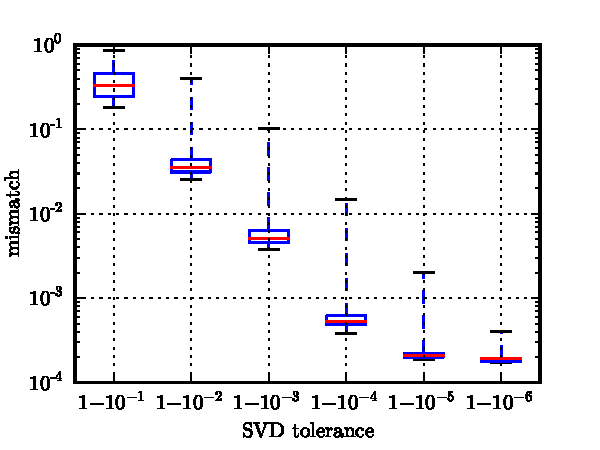
\includegraphics{figures/bw.pdf}}
	\subfloat[Mismatch versus $N^\shortuparrow$]{\label{fig:hist-interpolate}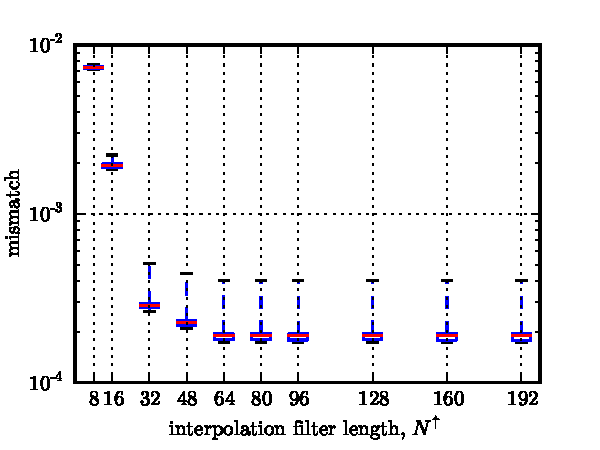
\includegraphics{figures/bw_resample.pdf}}
	\caption{Box-and-whisker plot of mismatch between nominal
template bank and \lloid\ measured impulse responses.  The upper and lower boundaries of
the boxes show the upper and lower quartiles; the lines in the center denote the medians.
The whiskers represent the minimum and maximum mismatch over all templates.  In 
\subref{fig:hist-svd-tolerance} the interpolation filter length is held fixed
at $N^\shortuparrow = 192$, while the \SVD\ tolerance is varied from
$\left(1-10^{-1}\right)$ to $\left(1-10^{-6}\right)$.  In \subref{fig:hist-interpolate}, the \SVD\ tolerance is fixed at $\left(1-10^{-6}\right)$ while $N^\shortuparrow$ is varied from 8 to 192 coefficients.}
\end{figure*}

\subsection{Lower bounds on computational cost compared to other methods}

We are now prepared to offer the estimated computational cost of filtering this
sub-bank of templates compared to other methods.  We used the results of the
previous subsections to set the \SVD\ tolerance to $1-10^{-4}$  and the
interpolation filter length to 16. Table \ref{table:flops} lists the
theoretical costs for filtering this sub-bank. Both the \FD\ method and \lloid\
are five orders of magnitude faster than the conventional \TD\ method.
However, the \FD\ method has a latency of over half of an hour, whereas \lloid\
has no latency at all.
%
\begin{table}
\caption{\label{table:flops}Computational cost in \flops\ of the \TD\ method, the \FD\ method, and \lloid\ for the bank of $2 \times 657$ templates sampled at 4096 Hz for chirp masses $1.1955 \leqslant \mathcal{M} / M_\odot \leqslant 1.2045$.  A block size of $D = 2 N$ is used for the \fft{}s in the \FD\ method.}
\begin{tabular}{lll}
\tableline\tableline
Method & \flops\ & Latency (s) \\
\tableline
Time domain (\TD) & $2.4\times10^{13}$ & 0 \\
Frequency domain (\FD) & $2.6\times10^8$ & 2201 \\
\lloid\ (this work) & $4.7\times10^8$ & 0 \\
\tableline
\end{tabular}
\end{table}

\subsection{Extrapolation of the computational cost to an Advanced \LIGO{} search}

Table~\ref{table:flops} shows that the \lloid\ method requires $\sim$$10^8$
\flops\ to cover a sub-bank comprising $\sim$$10^2$ out of the total $\sim$$10^5$
mass pairs.  Given that modern (ca. 2011) workstations can sustain computation
rates up to $\sim$$10^{10}$ \flops{}, and assuming that other regions of the
parameter space have similar computational scaling, an entire search could be
implemented with $\gtrsim$$10$ machines.  The lengths of templates does vary
over the parameter space; lower-mass templates are longer and would require
more computation to analyze while higher-mass templates are shorter and would
require less. However, we consider the estimates based on this sub-bank to be a
reasonable representation.

By comparison, using the \TD\ method to achieve the same latency costs
$\sim$$10^{13}$ \flops\ for this particular sub-bank, and so it would require
$\sim$$10^6$ present-day machines to search the full parameter space.
Presently, the \LIGO{} Data Grid consists of only $\sim$$10^4$ machines.


